\chapter{One gauge for a cell}\label{ch:gauge}

\section{The reading}

Every reading in this Part is an error score read on the same gauge: the reading divided by the same cell type's healthy
reading, on the same instrument,
\begin{equation}
  A=\frac{\text{reading}}{\text{healthy reference}} .
  \label{eq:A}
\end{equation}
$A=1$ is the cell working as itself and sits in the middle. Far below it lies $\Hmin$, the floor: where thermal kicks win against everything one ATP can buy
(Chapter~\ref{ch:iama}); nothing reads below it. The two ends of the gauge are fixed by physics: the floor by thermal kicks against one ATP,
the ceiling by a coin flip at every identity site. \derived{} Only the middle, the healthy reference, is measured, on purified healthy
cells of the same type (Chapter~\ref{ch:meta}). \measured{} Above 1 the cell makes more error than when healthy
(Figure~\ref{fig:gauge}). The ratio is dimensionless and independent of laboratory, array and person, provided the reading
and the reference are made on the same platform through the same calibration (Chapter~\ref{ch:instrument}). The same
construction reads qubits and chips in Part~\ref{part:3}; for a cell the healthy reference is the right standard,
because the question is whether this cell is still the cell it should be.

\begin{figure}[htbp]\centering
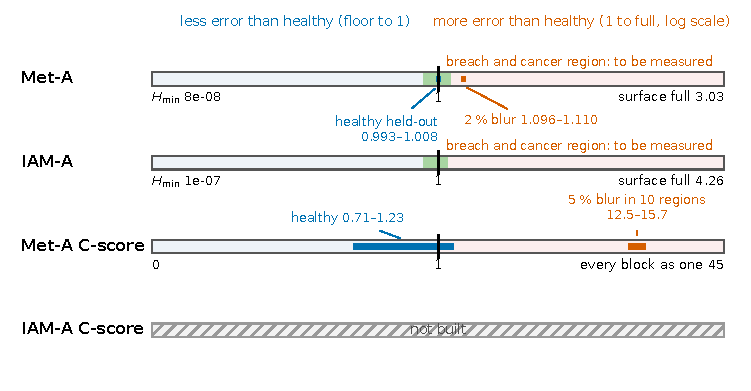
\includegraphics[width=\textwidth]{figures/part6/fig_gauge_cell.pdf}
\caption{One gauge, four readings, for neutrophils: Met-A (EPIC arrays), IAM-A (single molecules), the Met-A C-score and the IAM-A
C-score (not built). On every row 1 is the healthy reference, in the middle; the left half runs from the floor to 1 and the right half from 1 to
the far end on a log scale, so the two halves are not on one scale. Normal (green) is $0.95$--$1.05$. Bars are measured readings: held-out
healthy arrays, and the same arrays with known damage (Chapter~\ref{ch:skytools}). $\Hmin$, the floor where thermal kicks win against one ATP, is at $1\times10^{-7}$ on both rows, off the left edge. Breach and the cancer region lie to the right of Normal and are
to be measured on this scale. The surface is full when every identity site sits at a coin flip: $3.03$ (Met-A), $4.26$ (IAM-A).
The Met-A C-score sits on the same gauge: 1 is the healthy baseline, and its far end, every 50-site block moving as one, is 45. \calc}
\label{fig:gauge}
\end{figure}

\section{The points on the gauge}

\begin{center}\small
\begin{tabular}{@{}p{0.2\textwidth}p{0.2\textwidth}p{0.5\textwidth}@{}}\toprule
point & value (neutrophils) & status \\\midrule
$\Hmin$ & $1\times10^{-7}$ (IAM-A and Met-A) & \calc{} from $M$ alone: copy error $1/(1+e^{M})$ (Ch.~\ref{ch:iama}) \\
healthy reference & 1 (IAM-A $0.2348$ bits; Met-A $0.330263$ bits) & IAM-A \measured; Met-A \calibrated \\
Normal & $0.95$--$1.05$ & a design tolerance: healthy is $A=1\pm5$~\%; no group of people sets it \\
breach & to be measured & placed from per-person data: tumor/normal pairs, the DNMT1-inhibitor series, blood cancers \\
cancer region & beyond breach & to be measured the same way \\
full surface & Met-A $3.03$; IAM-A $4.26$ & \calc{} from the healthy reference alone \\
C-score far end & Met-A C-score $45$ & \calc{} block size 50 over the healthy baseline 1.1104; the IAM-A C-score is not built \\\bottomrule
\end{tabular}
\end{center}

\begin{keybox}[title=What the chain prints today]
Chain v3 prints the reading with one of three words: \emph{Normal}, \emph{above Normal}, \emph{below Normal}. Every line
beyond Normal is withheld until it is measured on this scale.
\end{keybox}

\section{The reading is an error rate}

At an identity site the cell holds methylated, a fraction $\varepsilon$ of its DNA copies has lost the mark and $\beta=1-\varepsilon$; at
a site it holds unmethylated, $\beta=\varepsilon$. Because $H(\beta)=H(1-\beta)$, the entropy at either site is the entropy of the error rate,
$H(\varepsilon)$. So
\begin{equation}
  A=\frac{H(\text{error now})}{H(\text{error in the same cell when healthy})},
\end{equation}
the cell's version of a qubit's gate error read against its specification. \derived{} $A=1$: errors at the healthy rate. $A>1$: more
errors; the pattern is blurring. $A<1$: fewer errors than healthy; the pattern is locking tighter.

\begin{center}\small
\begin{tabular}{@{}p{0.22\textwidth}p{0.3\textwidth}p{0.38\textwidth}@{}}\toprule
quantum computer & cell & what is measured \\\midrule
bit & one CpG on one DNA copy & methylated or not \\
intended state & the cell's identity pattern & the healthy reference \\
gate error & copy error at division (DNMT1 misses a site) & isolated unmethylated calls on single molecules (IAM-A) \\
$T_1$ decay & marks lost between divisions & region-wide loss; slow drift \\
leakage & writing where the pattern has none & gains on the unmethylated channel \\
error rate against specification & $A$ & $A$ per channel \\\bottomrule
\end{tabular}
\end{center}

\paragraph{One gauge, not one scale.} The gauge has the same shape everywhere: the system as built, or the cell when healthy, reads 1 in the
middle, its physical floor lies to the left and its full surface to the right. The distances do not carry from one system to another. $A=2$
for a neutrophil and $A=2$ for a qubit are both twice their reference, but the room between 1 and the full surface is different for each
(4.26 for a neutrophil on IAM-A), so equal readings do not mean equal damage, and the gauge does not rank systems against each other. Each
system is read against itself. \derived

Two cautions keep the mapping exact. First, Met-A measures \emph{state} error, the fraction of copies holding the wrong mark at one moment;
that is what copy error and decay leave behind together. Met-A says how much error there is; single-molecule reads say which process made
it. Second, the two channels can move in opposite directions, and a reading over both can hide both.

\paragraph{Two channels, read apart.} IMR90 lung fibroblasts (WGBS, GSE48580): three proliferating, three replicatively senescent and three
SV40-immortalized cultures, each read against the proliferating cultures, with the sites chosen on one proliferating culture and the
reference taken from a different one so that the reference is not computed on the data that chose the sites. \measured
\begin{center}\small
\begin{tabular}{@{}lccc@{}}\toprule
IMR90 & methylated channel & unmethylated channel & both \\\midrule
proliferating (held out) & 0.991--1.005 & 0.991--1.016 & 0.997--1.002 \\
senescent & 0.941--1.016 & 0.685--0.695 & 0.874--0.925 \\
SV40-immortalized & 1.077--1.120 & 0.587--0.664 & 0.965--0.975 \\\bottomrule
\end{tabular}
\end{center}
Senescent cells keep the methylated channel at the healthy rate and clean the unmethylated channel: fewer errors there, so the combined
reading sits below Normal. Immortalized cells do both at once, more error on the methylated channel and less on the unmethylated one, and the
two cancel: the combined reading, 0.965--0.975, sits inside Normal. A single number over both channels would call these cells healthy.

Figure~\ref{fig:p4_imr90} places every culture on the plane of the two channels.

\begin{figure}[htbp]\centering
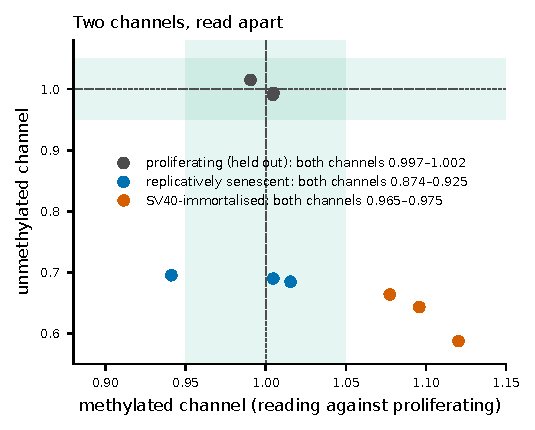
\includegraphics[width=0.62\textwidth]{figures/part6/fig_p4_06_imr90_channels.pdf}
\caption{IMR90 fibroblasts on the two channels (WGBS, GSE48580~\cite{Cruickshanks2013}), each culture read against the proliferating cultures, sites
and reference taken from different proliferating cultures. Shaded: Normal on each channel. Senescent cultures read 0.685--0.695 on the
unmethylated channel; SV40-immortalized cultures read 1.077--1.120 on the methylated channel and 0.965--0.975 on both together.
\measured}
\label{fig:p4_imr90}
\end{figure}
Channels are reported apart. Not yet checked: whether a difference in bisulfite conversion between the cultures contributes to the
unmethylated channel, where conversion failure reads as methylation (Chapter~\ref{ch:iama}). \openprob

\section{What healthy means, for each instrument}\label{sec:healthy}

Both instruments read a cell against its own healthy reference, but the two references are set differently. For Met-A the healthy
height is measured for each cell type. For IAM-A it starts from one physical number shared by all cell types, the holding energy, and one
measured correction places each cell type relative to it.

\begin{center}\small
\begin{tabularx}{\linewidth}{@{}>{\raggedright\arraybackslash}p{0.22\linewidth}>{\raggedright\arraybackslash}X>{\raggedright\arraybackslash}X@{}}
\toprule
 & Met-A & IAM-A \\\midrule
what is read & entropy $H(\beta)$ on the cell's identity sites, on arrays & copy error $\varepsilon$ on single molecules, by sequencing \\ \rowrule
what healthy is tied to & a measured height: $0.330263$ bits, the mean over six purified neutrophil arrays \measured & an energy shared by all cell types, $3.41\,\kB T$, which gives $\varepsilon_0=0.032$ \measured; then the cell type's position, $P_{\rm neutrophil}=1.149$ \measured \\ \rowrule
role of physics & fixes the two ends of the gauge \derived & fixes the two ends, and sets where healthy sits from one measured energy \derived \\ \rowrule
donors behind it & six (Salas~\cite{Salas2018}), screened healthy, aged 20--39 \observed & 153 public files of 56 healthy cell types for the energy; three granulocyte donors (Loyfer~\cite{Loyfer2023}), aged 50--56, for $P$ \observed \\ \rowrule
tested on cells that set nothing & other laboratories' healthy arrays read Normal (Chapter~\ref{ch:meta}) \measured & each donor read against the other two \measured; another laboratory's healthy cells not yet tested to a decision (its whole-blood test is incomplete: one library kit readable) \openprob \\ \bottomrule
\end{tabularx}
\end{center}

Because the IAM-A reference is anchored on an energy, IAM-A is the instrument that tests the law itself: a lever on the energy supply must
move it by the amount the law gives (Chapter~\ref{ch:development}). The energy $3.41\,\kB T$ is measured, not yet derived; deriving it from
the measured rates at which the copier restores and loses marks is the central open problem of the cellular rung (Chapter~\ref{ch:open}).
\openprob

\section{How far a reading moves}

What a reading can show depends on how far a real change moves it. On arrays, a simulated loss of 2~\% of the neutrophil
pattern in whole blood moves tared Met-A by about $+0.06$ (1.052--1.090 on six constructed mixtures); the shift scales with
the neutrophil fraction of the specimen, 0.033 at 40--50~\% neutrophils and 0.064 above 70~\%.
\measured{} On molecules, a simulated 2~\% rise in copy error moves IAM-A from about 1.00 to 1.29--1.35. \measured{} The
single-molecule reading is the more sensitive of the two by a factor of about five.

\section{The interval on a reading}

A reading carries three uncertainties. The healthy reference itself: six purified neutrophil arrays read one another, with
the identity sites re-chosen each time, at a standard deviation of 0.020 (Chapter~\ref{ch:meta}). The run: a same-run tare
against healthy references processed alongside the specimen states its own spread. And the fraction: in whole blood a cell
that is a small share of the DNA moves the reading less, so each specimen carries its own \emph{detection limit}, the
smallest loss of its neutrophil pattern it could show (Chapter~\ref{ch:chain}). \measured

\section{Three readings, in one sentence each}
\begin{itemize}
\item \textbf{Met-A} is reference metrology: information in bits, against a measured standard, the same cell type healthy.
\item \textbf{IAM-A} is the physics reading: copy error on single molecules against the floor set by thermal noise: a
holding energy of 3.41~$\kB T$ per site, which is 4.9 Landauer units ($3.41/\ln2$) and 0.16 of one ATP.
\item \textbf{The C-score} is a map statistic taken from cosmology: whether the departures are spread out or sit together in regions of the
genome (Chapter~\ref{ch:skytools}).
\end{itemize}

\section{Gauge words are not diagnoses}
\begin{rulebox}
A word on the gauge is a statement about where the error of a specimen's cells sits relative to the healthy cell of its kind. It
is not a diagnosis, a prognosis or a statement about a person. The report must not name conditions; the render-time guard that will enforce this on chain v3 is not yet built (Chapter~\ref{ch:report}).
\end{rulebox}
